\documentclass{article}
\usepackage[utf8]{inputenc}
\usepackage{amssymb,amsfonts,amsthm}
\usepackage{amsmath}
\usepackage{tikz}
\usepackage{framed}
\usepackage{multirow}
\usepackage[left=1in,right=1in,bottom=1in,top=1in]{geometry}
\usepackage{color}
\usepackage{hyperref}
\usepackage{titling}
\usepackage{graphicx}
\renewcommand\maketitlehooka{\null\mbox{}\vfill}
\renewcommand\maketitlehookd{\vfill\null}

\title{DeFi Data Engine Internal Manual}
\author{Conor Flynn}
\date{06/23/2022}

\begin{document}

% Title page
\maketitle
\cleardoublepage

% table of contents page
\tableofcontents


\cleardoublepage
\section{Abstract}
The DeFi Data Engine is an engine which serves as a gateway between data brokers and user interfaced applications. The engine is built to service data requests, historical data caching, and data distribution protocols all within a low latency, high frequency environment. This engine specifically caters to financial data, pertaining to asset prices, liquidity data, and exchange volume. Below is a high level model of the engine which will be expanded upon in Section 3 of this manual.

\begin{center}
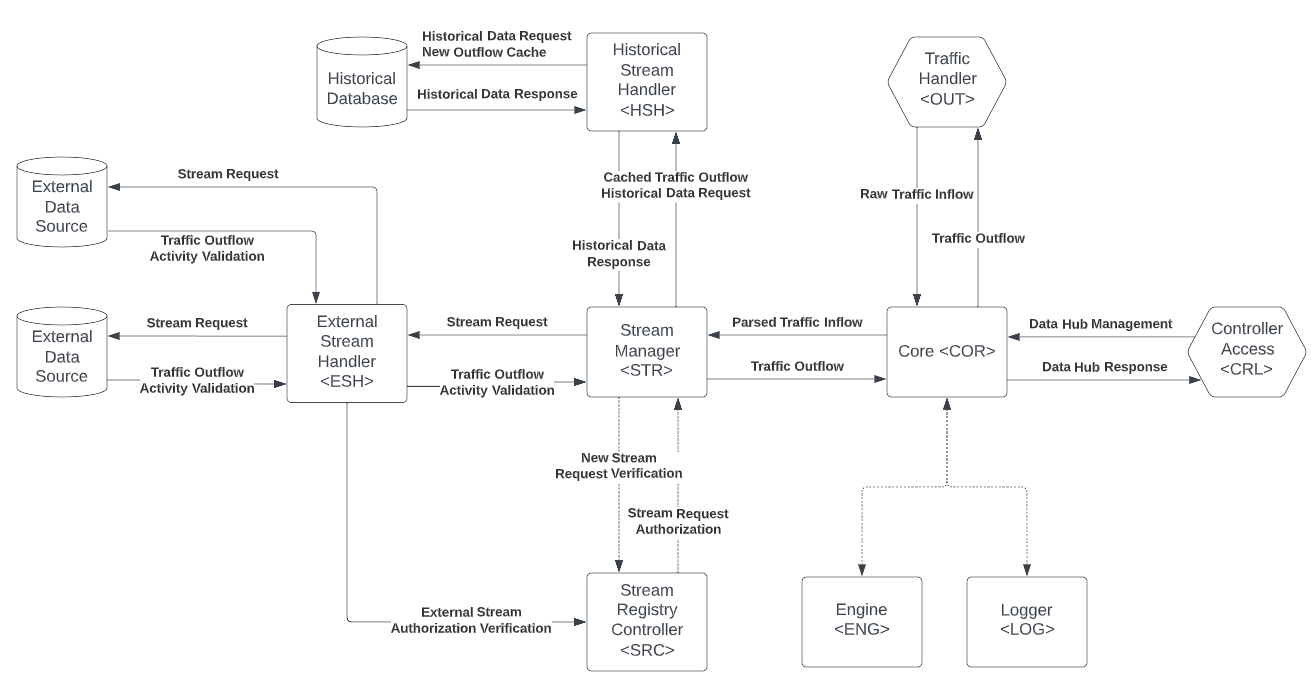
\includegraphics[scale=0.5]{data-core-framework}
\end{center}

%\cleardoublepage
\section{Stack}
This section describes the stack going to be used for this engine. Please make sure all pre-requisites are completed before attempting to use this engine in any capacity.

\subsection{Java}
Java SE 17 will be used for the development of the DeFi Data Engine. External libraries will be included in the build of the application and will be documented upon completion. All files will contain Java Docs as well for further development.\\

\underline{Prerequisites}

\begin{framed} 
Java JDK 17 Downloaded and Installed: 

-\;\href{https://www.oracle.com/java/technologies/downloads/#jdk17-windows}{https://www.oracle.com/java/technologies/downloads/\#jdk17\-windows}
\end{framed}

\subsection{Cap'n Proto}
Cap'n Proto is a data exchange format based on the RPC Protocol. It will be used for communication between the R Shiny application, DeFi Data Engine, and the Controller. The application was designed in C++ and therefore requires a development environment built to handle C++. Note this is ONLY required for development purposes and NOT required for use.


\cleardoublepage
\section{Data Core}
This section describes the data core of the engine, including an overview, component analysis, internal language, and internal connections.

\subsection{Overview}
The data core is a multi-threaded engine built for the handling of historical and live data streams. It will be able to accept requests through it's outside port and parse the specific requests to push data to the proper locations. 

Historical data will be stored within a database contained within the engine, and will be cached automatically via the live operating stream. Outside components can then request specific data from a historical time frame and the engine will automatically open a connection to the data base to feed in that stream.

Live data also can be requested through the engine, through a similar requesting process. Once requested, the data core will request authentication from the outside source to open the data stream. After authenticated successfully, a channel will be opened where all requested data will flow through.

All internal and external processes relating to the data core are documented below.

\subsection{Packets}
All external communication will use Cap'n Proto for the requesting and receiving of internal processes. To maintain consistency throughout calls only one object type will be accepted for these requests, called Packets. Packets will contain the format listed below, with the contents required of each section listed based on the needs of the engine.

\begin{center}
\begin{tabular}{ | p{3cm} || p{3cm} | p{9cm} | }
\hline
\multicolumn{3}{|c|}{Packet Formatting}\\
\hline
Name & Type & Description\\
\hline
Time & Long & NS Epoch time-stamp of packet when sent.\\
Destination & String & Packet destination.\\
Sender & String & Sender of the packet.\\
Tag & String & Request type of packet.\\
Sub-Tag & String & Additional Tag information. (optional)\\
Data & String & Data contained in packet.\\
\hline
\end{tabular}
\end{center}

\subsection{Controller Connection}
The controller is an external application that is used to monitor the engine's internal processes. It is connected via Cap'n Proto and allows for multiple requests and checks detailed below. Note these requests can also be made by other external applications however it is recommended against as it could hinder the speed of the engine.

Listed below are details relating to the identification of the Controller.

\begin{center}
\begin{tabular}{ | p{5cm} || p{4cm} | p{6cm} | }
\hline
\multicolumn{3}{|c|}{Controller Process Variables}\\
\hline
Name & Value & Description\\
\hline
UUID & controller\_process & Unique identifying name of the process.\\
\hline
Tag & CRL & Unique tag of the Controller process.\\
\hline
\end{tabular}
\end{center}

\subsubsection{Management}

The controller (and other external processes) will have the ability to request the following processes listed below. Processes refer to components within the engine which may require external monitoring for stability purposes. Description gives a short summary of the process being requested. Formatting of these requests will be listed in a later section.\\

\begin{center}
\begin{tabular}{ | p{5cm} || p{11cm} | }
\hline
\multicolumn{2}{|c|}{Management Requests}\\
\hline
Process & Description\\
\hline
Engine Start & Start engine processes.\\
\hline
Engine Kill & Force kill all engine processes.\\
\hline
Engine Active & Determines if the engine is currently active.\\
\hline
Engine Active Streams & List of all active streams being executed in the engine.\\
\hline
Log Request & Returns logs for given period if exists.\\
\hline
Log Stream & Opens stream of logs for processing.\\
\hline
Stream Exists & Determines if the stream has been requested by an external source at any time and has been stored within the active stream manager.\\
\hline
Stream Authorized & Checks if stream has been successfully authorized to start live data stream.\\
\hline
Stream Active & Determines if a stream is currently active. Does not have to be flowing data to return true.\\
\hline
Stream Last Call & Checks for the last time the stream saw a live data point flow through.\\ 
\hline
Historical Exists & Determines if historical data for specific type exists.\\
\hline
Historical Request & Returns historical data stored if exists.\\
\hline
\end{tabular}
\end{center}

\subsubsection{Request Formatting}
This section details all request formatting for calling the managerial processes listed in the prior section.

\begin{center}
\begin{tabular}{ | p{5cm} || p{2cm} | p{2cm} | p{6cm} | }
\hline
\multicolumn{4}{|c|}{Request Formatting}\\
\hline
Process & Tag & Sub-Tag & Data\\
\hline
Engine Start & ENG & STRT & N/A\\
\hline
Engine Kill & ENG & KILL & N/A\\
\hline
Engine Active & ENG & ACTV & N/A\\
\hline
Engine Active Streams & ENG & ACTS & N/A\\
\hline
Log Request & LOG & RQST & start\_epoch: $<$Long$>$\\
 &  &  & end\_epoch: $<$Long$>$\\
\hline
Log Stream & LOG & STRM & TBD\\
\hline
Stream Exists & STR & EXST & stream\_tag: $<$String$>$\\
\hline
Stream Authorized & STR & AUTH & stream\_tag: $<$String$>$\\
\hline
Stream Active & STR & ACTV & stream\_tag: $<$String$>$\\
\hline
Stream Last Call & STR & LCAL & stream\_tag: $<$String$>$\\
\hline
Historical Exists & HSH & EXST & start\_epoch: $<$Long$>$\\
 &  &  & end\_epoch: $<$Long$>$\\
 &  &  & time\_freq: $<$Long$>$\\
 &  &  & data\_category: $<$String$>$\\
\hline
Historical Request & HSH & RQST & start\_epoch: $<$Long$>$\\
 &  &  & end\_epoch: $<$Long$>$\\
 &  &  & time\_freq: $<$Long$>$\\
 &  &  & data\_category: $<$String$>$\\
\hline
\end{tabular}
\end{center}

\cleardoublepage
\subsubsection{Response Formatting}
This section details all response formatting for the managerial requests listed in the prior section.

\begin{center}
\begin{tabular}{ | p{5cm} || p{2cm} | p{2cm} | p{6cm} | }
\hline
\multicolumn{4}{|c|}{Response Formatting}\\
\hline
Process & Tag & Sub-Tag & Data\\
\hline
Engine Start & ENG & STRT & response\_code: $<$Long$>$\\
\hline
Engine Kill & ENG & KILL & response\_code: $<$Long$>$\\
\hline
Engine Active & ENG & ACTV & is\_active: $<$Boolean$>$\\
\hline
Engine Active Streams & ENG & ACTS & active\_streams: $<$String[]$>$\\
\hline
Log Request & LOG & RQST & logs: $<$String[]$>$\\
\hline
Log Stream & LOG & STRM & TBD\\
\hline
Stream Exists & STR & EXST & does\_exist: $<$Boolean$>$\\
\hline
Stream Authorized & STR & AUTH & is\_authorized: $<$Boolean$>$\\
\hline
Stream Active & STR & ACTV & is\_active: $<$Boolean$>$\\
\hline
Stream Last Call & STR & LCAL & last\_call: $<$Long$>$\\
\hline
Historical Exists & HSH & EXST & does\_exist: $<$Boolean$>$\\
\hline
Historical Request & HSH & RQST & returned\_data $<$String[]$>$\\ 
\hline
\end{tabular}
\end{center}

\subsection{Processes}
This section details all processes contained within the engine including: overview, functionality, and framework design.

\subsubsection{Router Superclass}
The Router is a super class that every process inherits. It is used to route data in a standardized manner throughout the engine. Each process that inherits the Router super class will be required to supply several types of information including: a UUID, a three-character tag, tags contained within the process, and routing tag information.

Listed below is information regarding the required information supplied above.

\begin{center}
\begin{tabular}{ | p{3cm} || p{3cm} | p{9cm} | }
\hline
\multicolumn{3}{|c|}{Router Parameters}\\
\hline
Name & Type & Description\\
\hline
UUID & String & Unique identifier of the inheriting process.\\
\hline
Tag & String & Unique tag of the inheriting process.\\
\hline
Contained Tags & String[] & All tags that will be processed within the inherited process.\\
\hline
Routed Tags & String[] & All tags that will be routed to other processes.\\
\hline
\end{tabular}
\end{center}

The Router also has several built in functions to handle the sending and receiving of Packet's between the processes. Listed below are all methods defined by the Router that will by used to send and receive packets. Please note that all methods passed in the Map objects must take a Packet as a parameter and return a Boolean.

\begin{center}
\begin{tabular}{ | p{5cm} || p{3cm} | p{7cm} | }
\hline
\multicolumn{3}{|c|}{Router Methods}\\
\hline
Method & Return & Description\\
\hline
Router(String, String, String[], String[]) & void & Base constructor for Router class. Defines all values stored within the Router class. Does not automatically connect any Router objects to self.\\
\hline
Router(String, String, String[], String[], Router[]) & void & Constructor for Router class. Defines all values stored within the Router class. Automatically connects all Router objects passed as a parameter such that individual function calls are not required.\\
\hline
getUUID() & String & Returns UUID provided in the constructor.\\
\hline
getTag() & String & Returns Tag provided in the constructor.\\
\hline
getContainedTags() & String[] & Returns Contained Tags provided in the constructor.\\
\hline
getRoutedTags() & String[] & Returns Routed Tags provided in the constructor.\\
\hline
getRouter(String) & Router & Returns connected Router object based on Tag sent as a parameter.\\
\hline
createPacket(String, String, String, String) & Packet & Helper function used to create a Packet object based off of the given parameters. Parameters are as follows: (Destination, Tag, Sub-Tag, Data).\\
\hline
connect(Router) & void & Connects Router object to Router passed as a parameter. Stores all connections and uses them for routing functions.\\
\hline
send(Packet) & Boolean & Sends Packet to connected Router object stored. Returns whether Packet was successfully sent. Throws error if destination does not exist in Router.\\
\hline
receive(Packet) & Boolean & Sends Packet to handler method based on method defined in constructor. Returns whether Packet was successfully processed.\\
\hline
abstract process(Packet) & Boolean & Router subclass function for handling incoming Packet objects.\\
\hline
\end{tabular}
\end{center}

\cleardoublepage
\subsubsection{Core}
The Core of the data engine will be the main router for traffic. This includes all incoming Packets from both the Controller as well as outside applications. All data will be subsequently logged and pushed to the proper locations from within the engine.

There are 3 main connections in and out of the core: the Traffic Handler, the Controller Access Point, and the Stream Manager.

Connection from the Traffic Handler will contain all incoming and outgoing processes, with all requests and responses documented in the Internal Language section. The Core also utilizes a Router super-class, which is the standard communication process for the engine and will be discussed in the Internal Language section.

Listed below are details relating to the identification of the Core.

\begin{center}
\begin{tabular}{ | p{5cm} || p{4cm} | p{6cm} | }
\hline
\multicolumn{3}{|c|}{Core Process Variables}\\
\hline
Name & Value & Description\\
\hline
UUID & core\_process & Unique identifying name of process.\\
\hline
Tag & COR & Unique tag of the Core process.\\
\hline
Contained Tags & ENG & All main engine controls.\\
& LOG & Logging functionality of the engine.\\
\hline
Routed Tags & STR & Routed to Stream Manager.\\
 & SRC & Routed to Stream Manager.\\
 & ESH & Routed to Stream Manager.\\
 & HSH & Routed to Stream Manager.\\
 & OUT & Routed to Traffic Handler.\\
 & CRL & Routed to Controller.\\
\hline
\end{tabular}
\end{center}

The Core will have several classes and files that are used to manage traffic and functions contained within it. Listed below are the different classes and their functions.

\begin{center}
\begin{tabular}{ | p{3cm} || p{4cm} | p{2cm} | p{6cm} | }
\hline
\multicolumn{4}{|c|}{Core Process Class Objects}\\
\hline
Class & Method & Return & Description\\
\hline
Core & Core() & void & Initializes the Core and defines all default values. Also initializes Router super class. Defines and initializes Logger, Engine, StreamManager, TrafficHandler, and ControllerHandler.\\
 & process(Packet) & boolean & Processes all incoming COR packets.\\
\hline
ENUM LogSeverity & INFO &  & Used for generic messages.\\
 & WARNING &  & Used for process warnings that may have impact on engine stability.\\
 & ERROR &  & Used for process errors that have critical impact on engine stability. Engine terminates immediately following an ERROR.\\
\hline
Logger & Logger(OutputStream) & void & Initializes Logger object with given output stream. Also initializes Router super class.\\
 & process(Packet) & boolean & Processes all LOG packets.\\
 & log(Object) & void & Pushes Object to OutputStream. Uses default LogSeverity of INFO.\\
 & log(LogSeverity, Object) & void & Pushes Object to OutputStream. Uses LogSeverity provided as a parameter.\\
\hline
Engine & Engine() & void & Initializes the Engine object. Also initializes Router super class.\\
 & process(Packet) & boolean & Processes all ENG packets.\\
 & start() & void & Starts internal clock and process stability manager.\\
 & stop() & void & Stops internal clock and stability manager.\\
\hline
\end{tabular}
\end{center}

\cleardoublepage
\subsubsection{Stream Manager}
The Stream Manager is the main processor for all stream requests, stream authorization, and stream handlers. This includes all stream request packets (external and historical), stream authorization packets, data return packets, and data caching packets.

There are 4 main connections in and out of the Stream Manager: the Core, the External Stream Handler, and the Historical Stream Handler. All request types and data formatting between these connections will be covered in the Internal Language section.

Listed below are details relating to the identification of the Stream Manager.

\begin{center}
\begin{tabular}{ | p{5cm} || p{4cm} | p{6cm} | }
\hline
\multicolumn{3}{|c|}{Core Process Variables}\\
\hline
Name & Value & Description\\
\hline
UUID & stream\_manager & Unique identifying name of process.\\
\hline
Tag & STR & Unique tag of the process.\\
\hline
Contained Tags & SRC & Stream Registry Controller process.\\
\hline
Routed Tags & ESH & Routed to External Stream Handler.\\
 & HSH & Routed to Historical Stream Handler.\\
 & OUT & Routed to Core.\\
 & CRL & Routed to Core.\\
 & ENG & Routed to Core.\\
 & LOG & Routed to Core.\\
\hline
\end{tabular}
\end{center}

The Stream Manager has several classes which control all processes and sub processes within this section of the engine. Listed below are the different classes and their functions.

\begin{flushleft}
\begin{center}
\begin{tabular}{ | p{3cm} || p{4cm} | p{2cm} | p{6cm} | }
\hline
\multicolumn{4}{|c|}{Stream Manager Process Class Objects}\\
\hline
Class & Method & Return & Description\\
\hline
StreamManager & StreamManager() & void & Initializes the StreamManager object and defines all of the necessary channels. Also initializes the Router super class. Defines and initializes ExternalStreamHandler, HistoricalStreamHandler, and StreamRegistryController.\\
 & process(Packet) & boolean & Processes all STR packets.\\
\hline
StreamRegistry-Controller & StreamRegistryController() & void & Initializes the StreamRegistryController object and the Router super class.\\
 & process(Packet) & boolean & Processes all SRC packets.\\
 & exists(String) & boolean & Returns whether a Stream with given tag exists in the registry.\\
 & authorized(String) & boolean & Returns whether a Stream contains the proper authorization credentials to start.\\
 & active(String) & boolean & Returns whether a Stream with the given tag is active.\\
 & execute(Packet) & boolean & Executes a Stream based off of the passed information. Validates all required information prior to execution.\\
 & register(Packet) & void & Registers a stream into the registry to track activity.\\
 & update(Packet) & void & Updates the status of a stream based on transferred packet.\\
\hline

\end{tabular}
\end{center}
\end{flushleft}

\cleardoublepage
\subsubsection{External Stream Handler}
The External Stream Handler is the main hub for all integrated data sources. Here, requests are processed and sent to the requested sources and then data streams are opened and sent to the outside sources. Requests must first be processed and authorized in the Stream Registry Controller before being sent.

Listed below are details relating to the identification of the Stream Manager.

\begin{center}
\begin{tabular}{ | p{5cm} || p{4cm} | p{6cm} | }
\hline
\multicolumn{3}{|c|}{External Stream Handler Process Variables}\\
\hline
Name & Value & Description\\
\hline
UUID & external\_stream\_manager & Unique identifying name of process.\\
\hline
Tag & ESH & Unique tag of the process.\\
\hline
Contained Tags & & \\
\hline
Routed Tags & SRC & Routed to Stream Registry Controller.\\
 & OUT & Routed to Traffic Handler.\\
\hline
\end{tabular}
\end{center}

The External Stream Manager has several classes which control all processes and sub processes within this section of the engine. There is also an abstract class which all outside sources are required to implement and handle should they want to be recognized by the engine.

\begin{flushleft}
\begin{center}
\begin{tabular}{ | p{3cm} || p{4cm} | p{2cm} | p{6cm} | }
\hline
\multicolumn{4}{|c|}{Stream Manager Process Class Objects}\\
\hline
Class & Method & Return & Description\\
\hline
ExternalStream- Handler & ExternalStreamHandler() & void & Initializes the ExternalStreamHandler object and defines all necessary channels. Also initializes the Router super class. Uses Reflections library to recognize all outside data sources compatible with the engine as to not require manual integration.\\
 & process(Packet) & boolean & Processes all ESH packets and sends requests to appropriate outside sources.\\
\hline
ABSTRACT ExternalConnection & ExternalConnection() & void & Initializes the outside connection class, defining all necessary variables.\\
 & final const SOURCE & String & Required unique source id of the outside source. Used by engine to identify external connection.\\
 & getSource() & String & Returns unique source id.\\
 & process(Packet) & boolean & Function used to process data packets sent by ESH.\\
 & abstract authorize(Packet) & boolean & Used to authorize connection.\\
 & abstract isAuthorized() & boolean & Used to confirm authorization.\\ 
 & abstract valid(Packet) & boolean & Used to confirm that request is valid to send.\\
 & abstract request(Packet) & boolean & Sends request for data to connection.\\
\hline

\end{tabular}
\end{center}
\end{flushleft}

\cleardoublepage
\subsubsection{Historical Stream Handler}
The Historical Stream Handler is the main hub for all historically cached data. Outside sources can make requests for cached data to then use for various processes. Externally sourced data is also cached here real time to reduce latency when requesting historical data. All requests are first validated through the Stream Registry Controller before being submitted.

Listed below are details relating to the identification of the Historical Stream Manager.

\begin{center}
\begin{tabular}{ | p{5cm} || p{4cm} | p{6cm} | }
\hline
\multicolumn{3}{|c|}{Historical Stream Handler Process Variables}\\
\hline
Name & Value & Description\\
\hline
UUID & historical\_stream\_manager & Unique identifying name of process.\\
\hline
Tag & HSH & Unique tag of the process.\\
\hline
Contained Tags & & \\
\hline
Routed Tags & SRC & Routed to Stream Registry Controller.\\
 & OUT & Routed to Traffic Handler.\\
\hline
\end{tabular}
\end{center}

\textbf{Functions within the Historical Stream Handler are TBH due to the current design being undecided.}

\cleardoublepage
\subsection{Internal Language}
The Internal Language section will discuss how managerial processes are executed, how to request streams from within the application, and how to manage data outflow.

\subsubsection{Management Processes}
Please reference section 3.3.1 for all Management Process requests. This section will most likely be expanded in later versions.

\subsubsection{External Stream Requests}
External Stream Requests are requests made the External Stream Handler to subscribe to a live data feed. Each of these requests is first processed through the Stream Registry Control before being sent to the External Stream Handler.

The general flow of the an External Stream Request is listed as follows.

\begin{flushleft}
\begin{center}
\begin{tabular}{ | p{1cm} || p{2cm} | p{2cm} | p{2cm} | p{2cm} | p{6cm} | }
\hline
\multicolumn{6}{|c|}{External Stream Request Path}\\
\hline
Step & Sender & Responder & Tag & Sub-Tag & Description\\
1. & OUT & COR & SRC & EXEC & Transit from OUT to COR.\\
2. & COR & STR & SRC & EXEC & Transit from COR to STR.\\
3. & STR & SRC & SRC & EXEC & Transit from STR to SRC.\\
4. & SRC &  -  & SRC & EXEC & Process request and send authorization to ESH.\\
5. & SRC & STR & ESH & AUTH & Transit from SRC to STR.\\
6. & STR & ESH & ESH & AUTH & Transit from STR to ESH.\\
7. & ESH &  -  & ESH & AUTH & Authorize stream and reply with response code to SRC.\\
8. & SRC &  -  &  -  &  -   & Process response code from ESH.\\
9a. & SRC & OUT &  -  &  -   & If invalid response from ESH, return response code to OUT.\\
9b. & SRC & STR & ESH & EXEC & If valid response from ESH, send execution packet to ESH. Transit from STR to SRC.\\
10. & STR & ESH & ESH & EXEC & Transit from STR to ESH.\\
11. & ESH &  -  & ESH & EXEC & Process execution packet and open stream on provided channel.\\
12. & ESH & STR & OUT & EDAT & Data packet from ESH to OUT. Transit from ESH to STR.\\
13. & STR & COR & OUT & EDAT & Transit from STR to COR.\\
14. & COR & OUT & OUT & EDAT & Transit from COR to OUT.\\
15. & OUT &  -  & OUT & EDAT & Submit data packet to outside source.\\ 
\hline
\end{tabular}
\end{center}
\end{flushleft}


\cleardoublepage
\subsubsection{Historical Stream Requests}

\begin{flushleft}
\begin{center}
\begin{tabular}{ | p{1cm} || p{2cm} | p{2cm} | p{2cm} | p{2cm} | p{6cm} | }
\hline
\multicolumn{6}{|c|}{External Stream Request Path}\\
\hline
Step & Sender & Responder & Tag & Sub-Tag & Description\\
1. & OUT & COR & SRC & HRQS & Transit from OUT to COR.\\
2. & COR & STR & SRC & HRQS & Transit from COR to STR.\\
3. & STR & SRC & SRC & HRQS & Transit from STR to SRC.\\
4. & SRC &  -  & SRC & HRQS & Process request and send validation request to HSH.\\
5. & SRC & STR & HSH & EXDT & Send request to see if data exists in database. Transit from SRC to STR.\\
6. & STR & HSH & HSH & EXDT & Transit from STR to HSH.\\
7. & HSH &  -  & HSH & EXDT & Validate data exists and send response code to SRC.\\
8. & SRC &  -  &  -  &  -   & Process response code from HSH.\\
9a. & SRC & OUT &  -  &  -   & If invalid response from HSH, return response code to OUT.\\
9b. & SRC & STR & HSH & HRQS & If valid response from HSH, send data request to HSH. Transit from SRC to STR.\\
10. & STR & HSH & HSH & HRQS & Transit from STR to HSH.\\
11. & HSH &  -  &  HSH & HRQS & Process request packet and send data to OUT on provided channel.\\
12. & HSH & STR & OUT & HDAT & Data packet from HSH to OUT. Transit from HSH to STR.\\
13. & STR & COR & OUT & HDAT & Transit from STR to COR.\\
14. & COR & OUT & OUT & HDAT & Transit from COR to OUT.\\
15. & OUT &  -  & OUT & HDAT & Submit data packet to outside source.\\

\hline
\end{tabular}
\end{center}
\end{flushleft}

\end{document}